%
% ========================================================================
%
%  	
%
%   Authors: 
%   Created: Jan, 2012.
%
% ========================================================================
% ----------------------------------
%  Class and Packages
% ----------------------------------

%\documentclass[portait,custom]{sciposter}
\documentclass[landscape,custom]{sciposter}

% ----------------------------------
%  Customization and Macros
% ----------------------------------

\usepackage{local}

%\usepackage{hyperref}
%\hypersetup{colorlinks=true,citecolor=black,filecolor=black,linkcolor=black,urlcolor=black,breaklinks=true}
\usepackage{supertabular}
\usepackage{rotating,multirow}
%\usepackage{soul}
\usepackage[multidot]{grffile}
\usepackage{dcolumn}
\newcolumntype{s}{D{.}{.}{1.2}}
\usepackage{natbib}
\bibpunct{(}{)}{;}{a}{,}{,~}
%\usepackage[comma,sort]{natbib}
%\bibliographystyle{plainnat}

\usepackage{comment}

\usepackage{sectionbox}

% ========================================================================
\leftlogo{
\hspace*{-0.01in}
            \raisebox{-100pt}{\begin{minipage}[c]{5.0in}\centering
	    
\includegraphics[width=\columnwidth]{logos/ORNL_logo.pdf}
           %\includegraphics[width=\columnwidth]{logos/RUBISCO_logo_for_posters.eps} \\
           %vskip-0.35in
\includegraphics[width=\columnwidth]{logos/CCSI_Text_Logo_transparent.png}%
\end{minipage}
%\hspace*{-0.85in}
}

            %\hspace*{12pt}
            %\raisebox{-265pt}{
\includegraphics[height=2.00in]{logos/CCSI_Text_Logo_transparent.png}}%
            %%\hspace*{25pt}%
            %%\raisebox{-190pt}{
\includegraphics[height=2.00in]{logos/CCSI_logo_FMH.pdf}}%
}
\rightlogo{
\hspace*{-4.0in} 
           \hspace*{-4.0in}
           \raisebox{-100pt}{\begin{minipage}[c]{6.0in}\centering
            %
\includegraphics[width=\columnwidth]{logos/uci_peter.png} \\
            %\vskip-0.35in 
            %
\includegraphics[width=\columnwidth]{logos/ess_logo_white.pdf}
            
\includegraphics[width=\columnwidth]{logos/CCSI_Text_Logo_transparent.png}%
\end{minipage}
}
}

\newcommand{\VERYHUGE}{\fontsize{80.00}{20.00}\selectfont}

% AGU 2014 Poster Title
%\title{\VERYHUGE \vbox{\fbox{GC41C-0573} Long-term Terrestrial Carbon and Water Cycle Responses to Projected Climate Change Beyond 2100}}
% CCSI SAB Poster Title
%\title{\VERYHUGE \vbox{Long-term Terrestrial Carbon and Water Cycle Responses to Projected Climate Change Beyond 2100}}
% AGU 2015 Poster Title
%\title{\VERYHUGE\color{RUBISCO-DarkSlateBlue} \vbox{Nonlinear Interactions between Climate and Atmospheric Carbon Dioxide Drivers of Terrestrial and Marine Carbon Cycle Changes from 1850 to 2300}}
\title{\VERYHUGE\color{RUBISCO-DarkSlateBlue} \vbox{Quantifying Feedbacks of Climate Intervention Under Climate Change}}

\author{%\normalsize
  Forrest~M.~Hoffman$\mbox{}^\textnormal{1}$,
  Min~Xu$\mbox{}^\textnormal{1}$,
  Wei~Zhang$\mbox{}^\textnormal{1}$,
  Salil~Mahajan$\mbox{}^\textnormal{1}$,
  Xiaojuan~Yang$\mbox{}^\textnormal{1}$,
  Cheng-En~Yang$\mbox{}^\textnormal{2}$,
  and
  the~Climate~Intervention~Biology~Working~Group
  }


% institute name
\institute{\small
  %$\mbox{}^\textnormal{1}$Department of Earth System Sciences, University of California, Irvine, California 92697, USA;
  $\mbox{}^\textnormal{1}$Climate Change Science Institute, Oak Ridge National Laboratory, Oak Ridge, Tennessee 37831, USA; \\
  %$\mbox{}^\textnormal{3}$Department of Atmospheric Sciences and Department of Biology, University of Washington, Seattle, WA~98195-1640, USA;
  %$\mbox{}^\textnormal{4}$Earth Sciences Division, Lawrence Berkeley National Laboratory, Berkeley, CA~94720, USA; \\
  %$\mbox{}^\textnormal{5}$Earth and Atmospheric Sciences, Cornell University, Ithaca, New York 14853, USA;
  %$\mbox{}^\textnormal{6}$Climate \& Global Dynamics Division, National Center for Atmospheric Research, Boulder, Colorado 80307, USA
  and
  $\mbox{}^\textnormal{2}$Department of Civil \& Environmental Engineering, University of Tennessee, Knoxville, Tennessee 37996, USA
}

% ========================================================================
\setmargins[2cm]

\begin{document}

\conference{Conference on Innovations in Climate Resilience (March 29--30, 2022), Columbus, Ohio, USA \hfill Oak Ridge National Laboratory (ORNL) is managed by UT-Battelle, LLC, for the U.S.\ Department of Energy under contract DE-AC005-00OR22725.}

\vspace*{0.5in}
\maketitle

% For the SciDAC3 PI Meeting, we are forbidden to use any DOE logos!
%\includegraphics[height=1.25in]{logos/ANL_logo}\hfill\includegraphics[height=1.25in]{logos/LLNL_logo}\hfill\includegraphics[height=1.25in]{logos/LANL_logo}\hfill\includegraphics[height=1.25in]{logos/NCAR_logo}\hfill
\includegraphics[height=1.25in]{logos/ORNL_logo}\hfill\includegraphics[height=1.25in]{logos/PNNL_logo}\hfill\includegraphics[height=1.25in]{logos/SNL_logo}

\vspace*{-0.75in}

\begin{multicols}{4}

%%%%%%%%%%%%%%%%%%%%%%%%%%%%%%%%%%%%%%%%%%%%%%%%%%%%%%%%%%%%%%%%%%%%%%%%%%%%%%%
\section*{\large Introduction}
%%%%%%%%%%%%%%%%%%%%%%%%%%%%%%%%%%%%%%%%%%%%%%%%%%%%%%%%%%%%%%%%%%%%%%%%%%%%%%%

\begin{itemize}

\item The increasing severity of the effects of climate change, especially strengthening extreme events and wildfire, is theatening built infrastructure, utilities, and national and economic security.

\item Loss of life and property is motivating serious consideration of approaches for \textbf{climate intervention} or \textbf{geoengineering}.

\item In addition to efforts to scale up \textbf{carbon dioxide removal (CDR)} through \textbf{direct air capture (DAC)} and other means, interest in growing in methods to reduce or stabilize Earth's surface temperature.

\item \textbf{Solar radiation management (SRM)} is one approach to partially reduce warming by reflecting a portion of incoming solar radiation to maintain resilience of the Earth system.

\item \textbf{Stratospheric aerosol intervention (SAI)}, through direct injection of sulfur into the lower stratosphere, is considered the most feasible scheme.

\item Many questions remain unanswered regarding the feedback effects of SAI on the Earth system.

\end{itemize}

\begin{figure}
	\begin{center}
		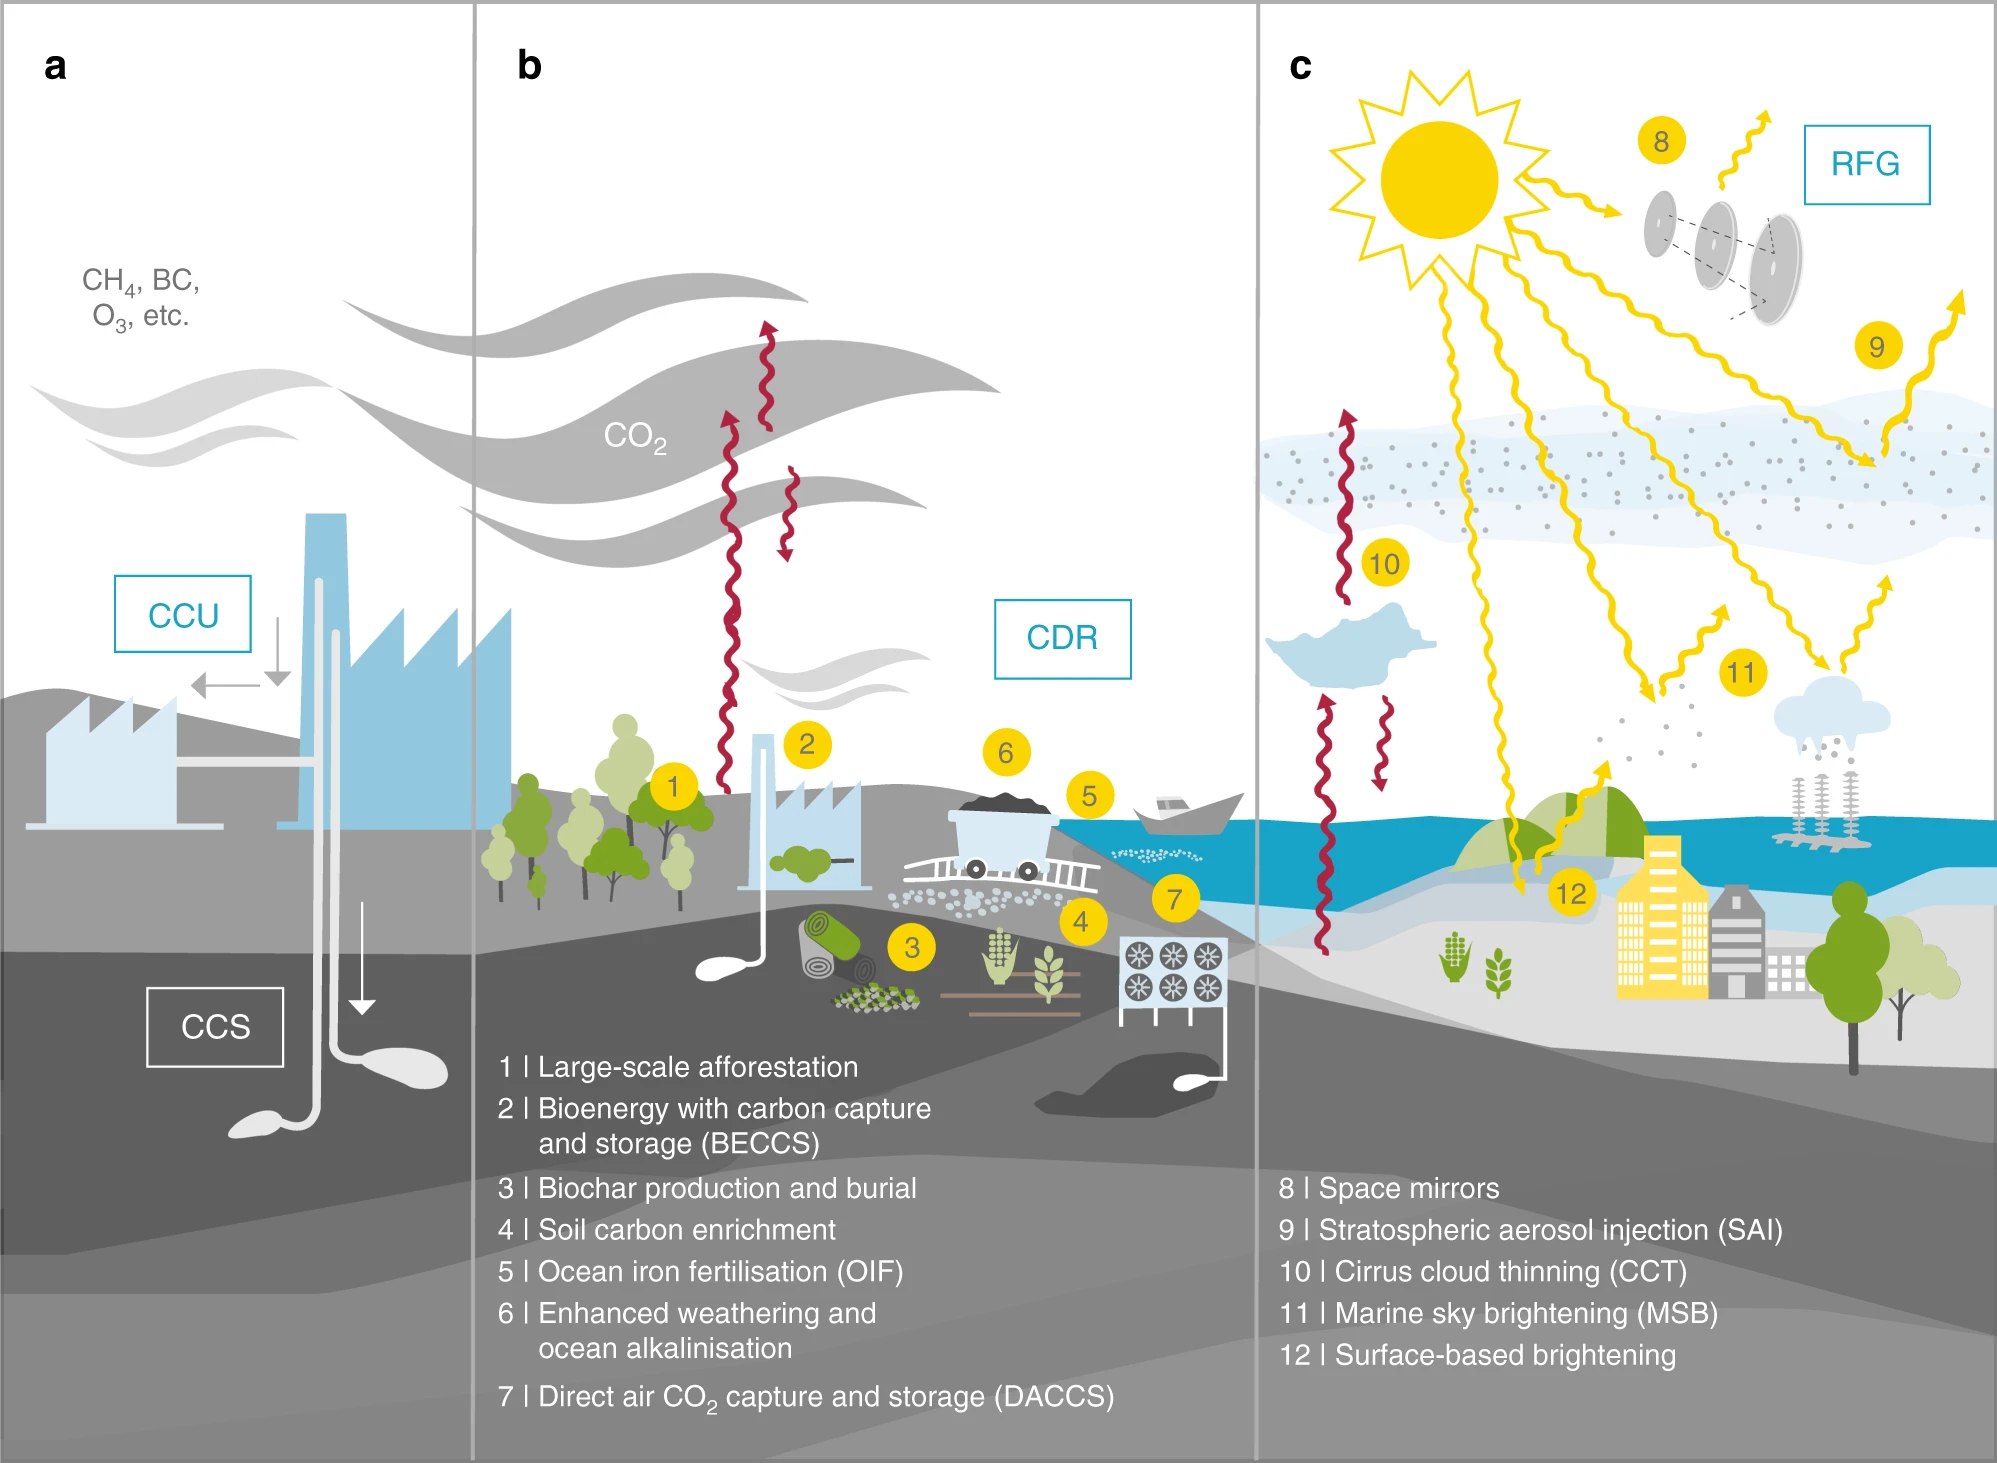
\includegraphics[width=0.8\columnwidth]{figures/41467_2018_5938_Fig1_HTML.png}
	\end{center}
	\caption{Proposed climate geoengineering techniques placed in the context of mitigation efforts. Adopted from Lawrence et al. (2018).
		% https://www.nature.com/articles/s41467-018-05938-3
	}
\end{figure}


%%%%%%%%%%%%%%%%%%%%%%%%%%%%%%%%%%%%%%%%%%%%%%%%%%%%%%%%%%%%%%%%%%%%%%%%%%%%%%%
\section*{\large Potential Ecological Impacts of Climate Intervention}
%%%%%%%%%%%%%%%%%%%%%%%%%%%%%%%%%%%%%%%%%%%%%%%%%%%%%%%%%%%%%%%%%%%%%%%%%%%%%%%

\begin{itemize}
	\item While climate science research has focused on predicted climate effects of SRM, \textbf{few studies have investigated impacts that SRM would have on ecological systems}.
	\item Impacts and risks posed by SRM would vary by implementation scenario, anthropogenic climate effects, geographic region, and by ecosystem, community, population, and organism.

\end{itemize}

\begin{figure}
	\begin{center}
		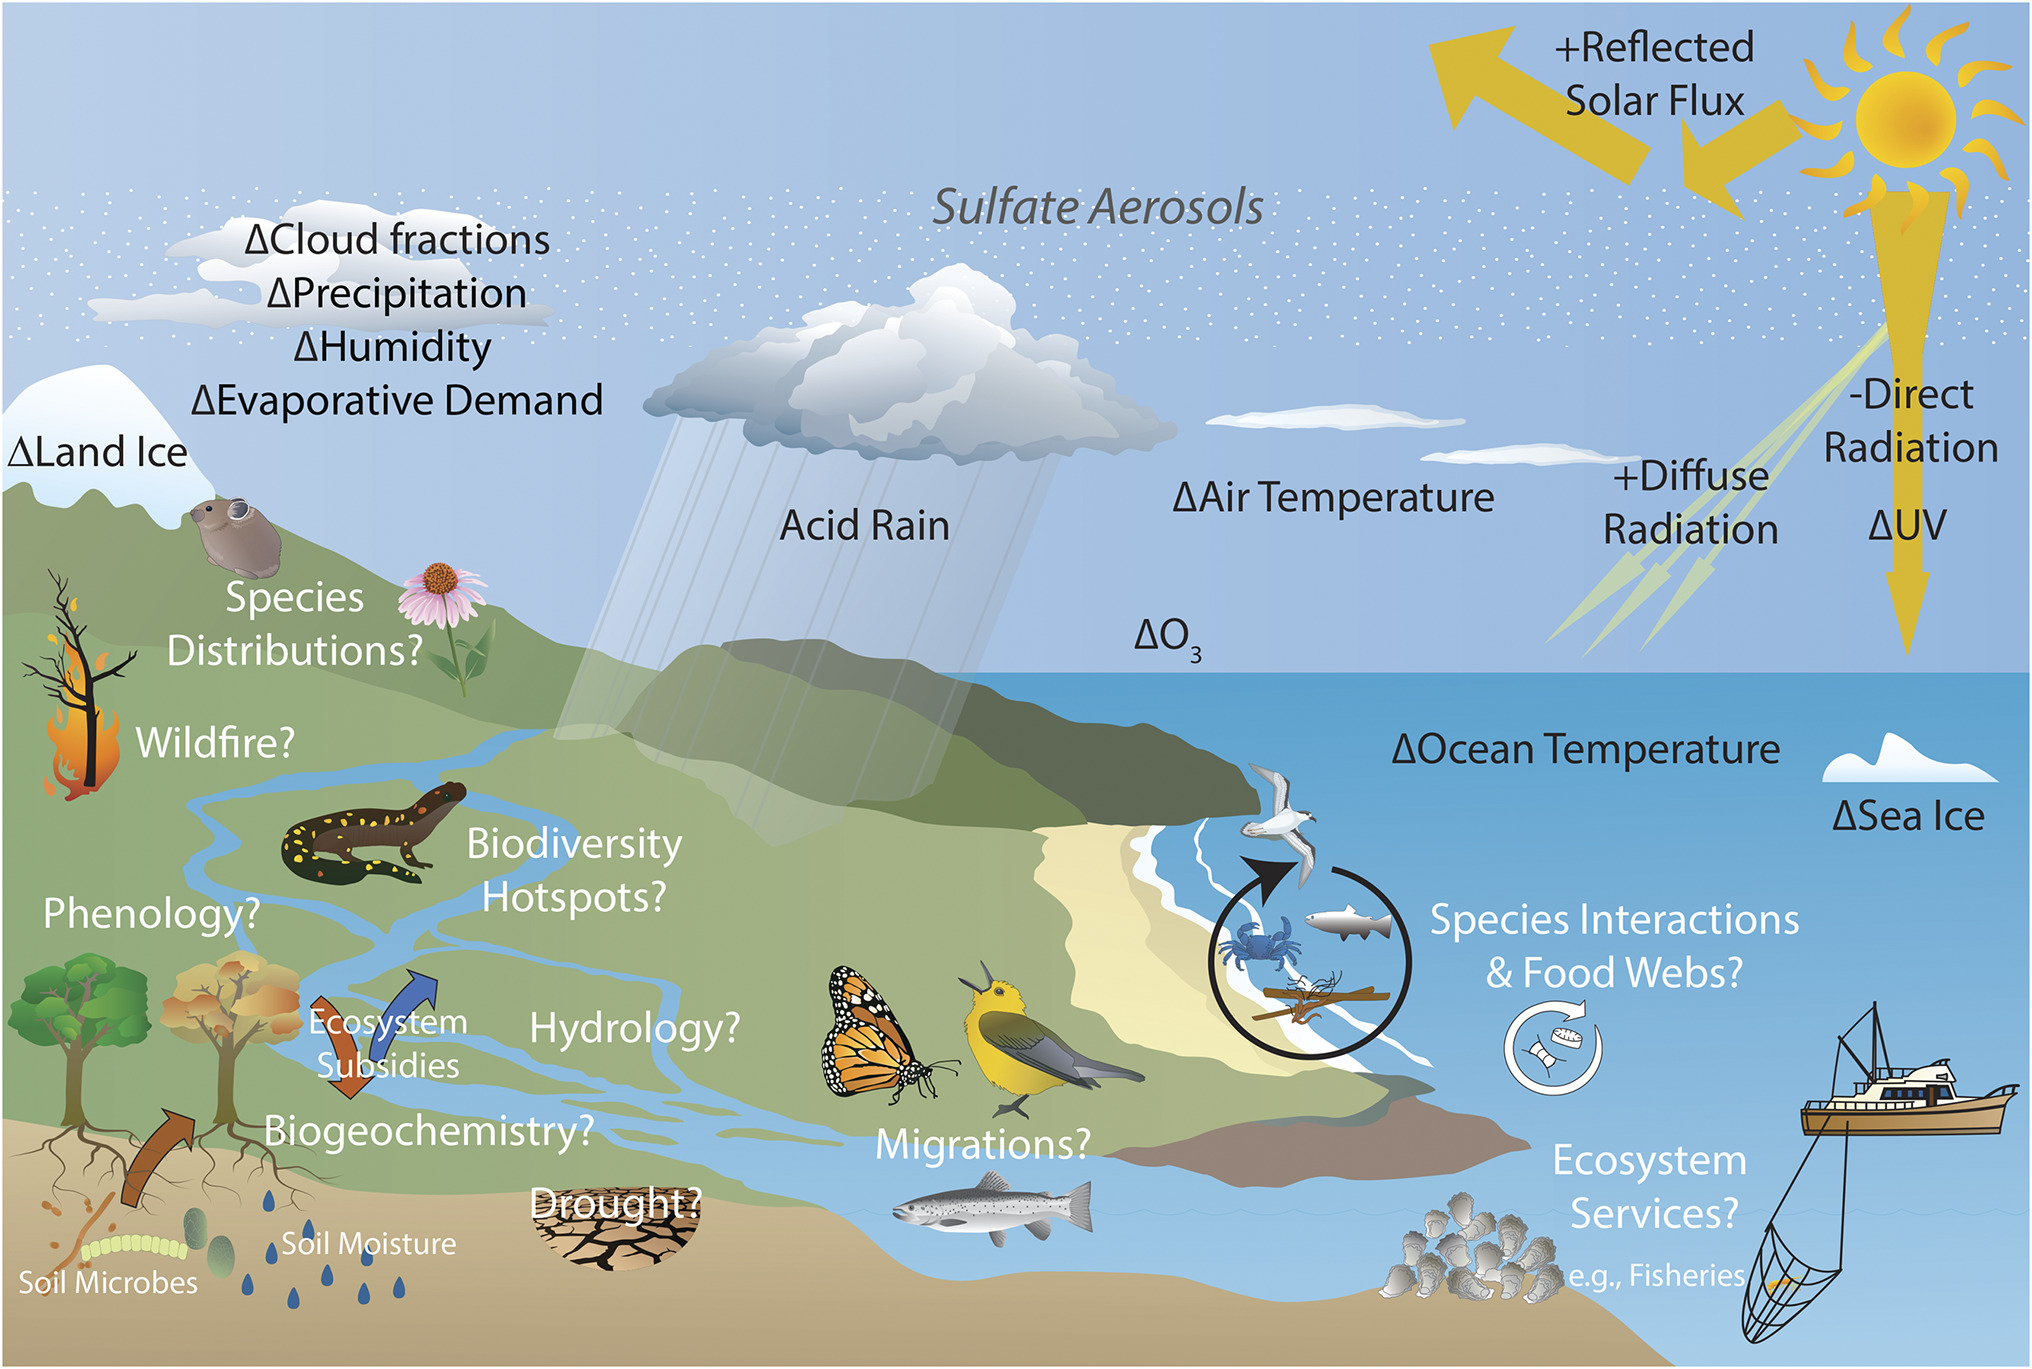
\includegraphics[width=0.8\columnwidth]{figures/pnas.1921854118fig01.jpg}
	\end{center}
	\caption{Although some effects of SRM with SAI on the climate are known from certain SAI scenarios (indicated with $+$ for likely increases, $-$ for decreases, $\Delta$ to indicate change), the effects of SAI on ecological systems are largely unknown. Adopted from Zarnetske et al. (2021).
		% https://www.pnas.org/doi/10.1073/pnas.1921854118
	}
\end{figure}

\begin{itemize}
	\item Models used for projecting responses to SAI are often the same Earth system models (ESMs) used to study anthropogenic climate change effects without SAI.
	\item These models must additionally be able to represent complex stratospheric aerosol processes and ecological responses and feedbacks.

	\item \textbf{A transdisciplinary approach, increasing collaboration between ecologists and climate scientists, is essential} for understanding the benefits and risks of SAI on climate and to ecological systems.
\end{itemize}



%%%%%%%%%%%%%%%%%%%%%%%%%%%%%%%%%%%%%%%%%%%%%%%%%%%%%%%%%%%%%%%%%%%%%%%%%%%%%%%
\section*{\large Terrestrial Biogeochemical Feedbacks In a Strategically Geoengineered Climate}
%%%%%%%%%%%%%%%%%%%%%%%%%%%%%%%%%%%%%%%%%%%%%%%%%%%%%%%%%%%%%%%%%%%%%%%%%%%%%%%


\begin{itemize}
	\item To characterize terrestrial ecosystem (vegetation and soil) responses and feedbacks resulting from SAI, we analyzed an ensemble of global coupled ESM climate change simulations.
	\item The simulations employed the Community Earth System Model (CESM) and were performed for the Stratospheric Aerosol Geoengineering Large Ensembe (GLENS) project at the National Center for Atmospheric Research (NCAR).
	\item The ensemble simulations followed the Fifth Phase Coupled Model Intercomparison Project (CMIP5) Historical and RCP8.5 simulations from 1850--2100.
	\item The baseline experiment period, called \textbf{\textit{BASE}}, ran for 2010--2019, and the control, called \textbf{\textit{CTRL}}, ran for 2020--2097, following the standard CMIP6 protocol.
	\item A third set of ensemble members, called \textbf{\textit{GEOENG}}, ran for 2020-2097 with simulated SAI mitigation designed to stabilize global temperatures at those for the year 2020.

\end{itemize}


\begin{figure}
	\begin{center}
		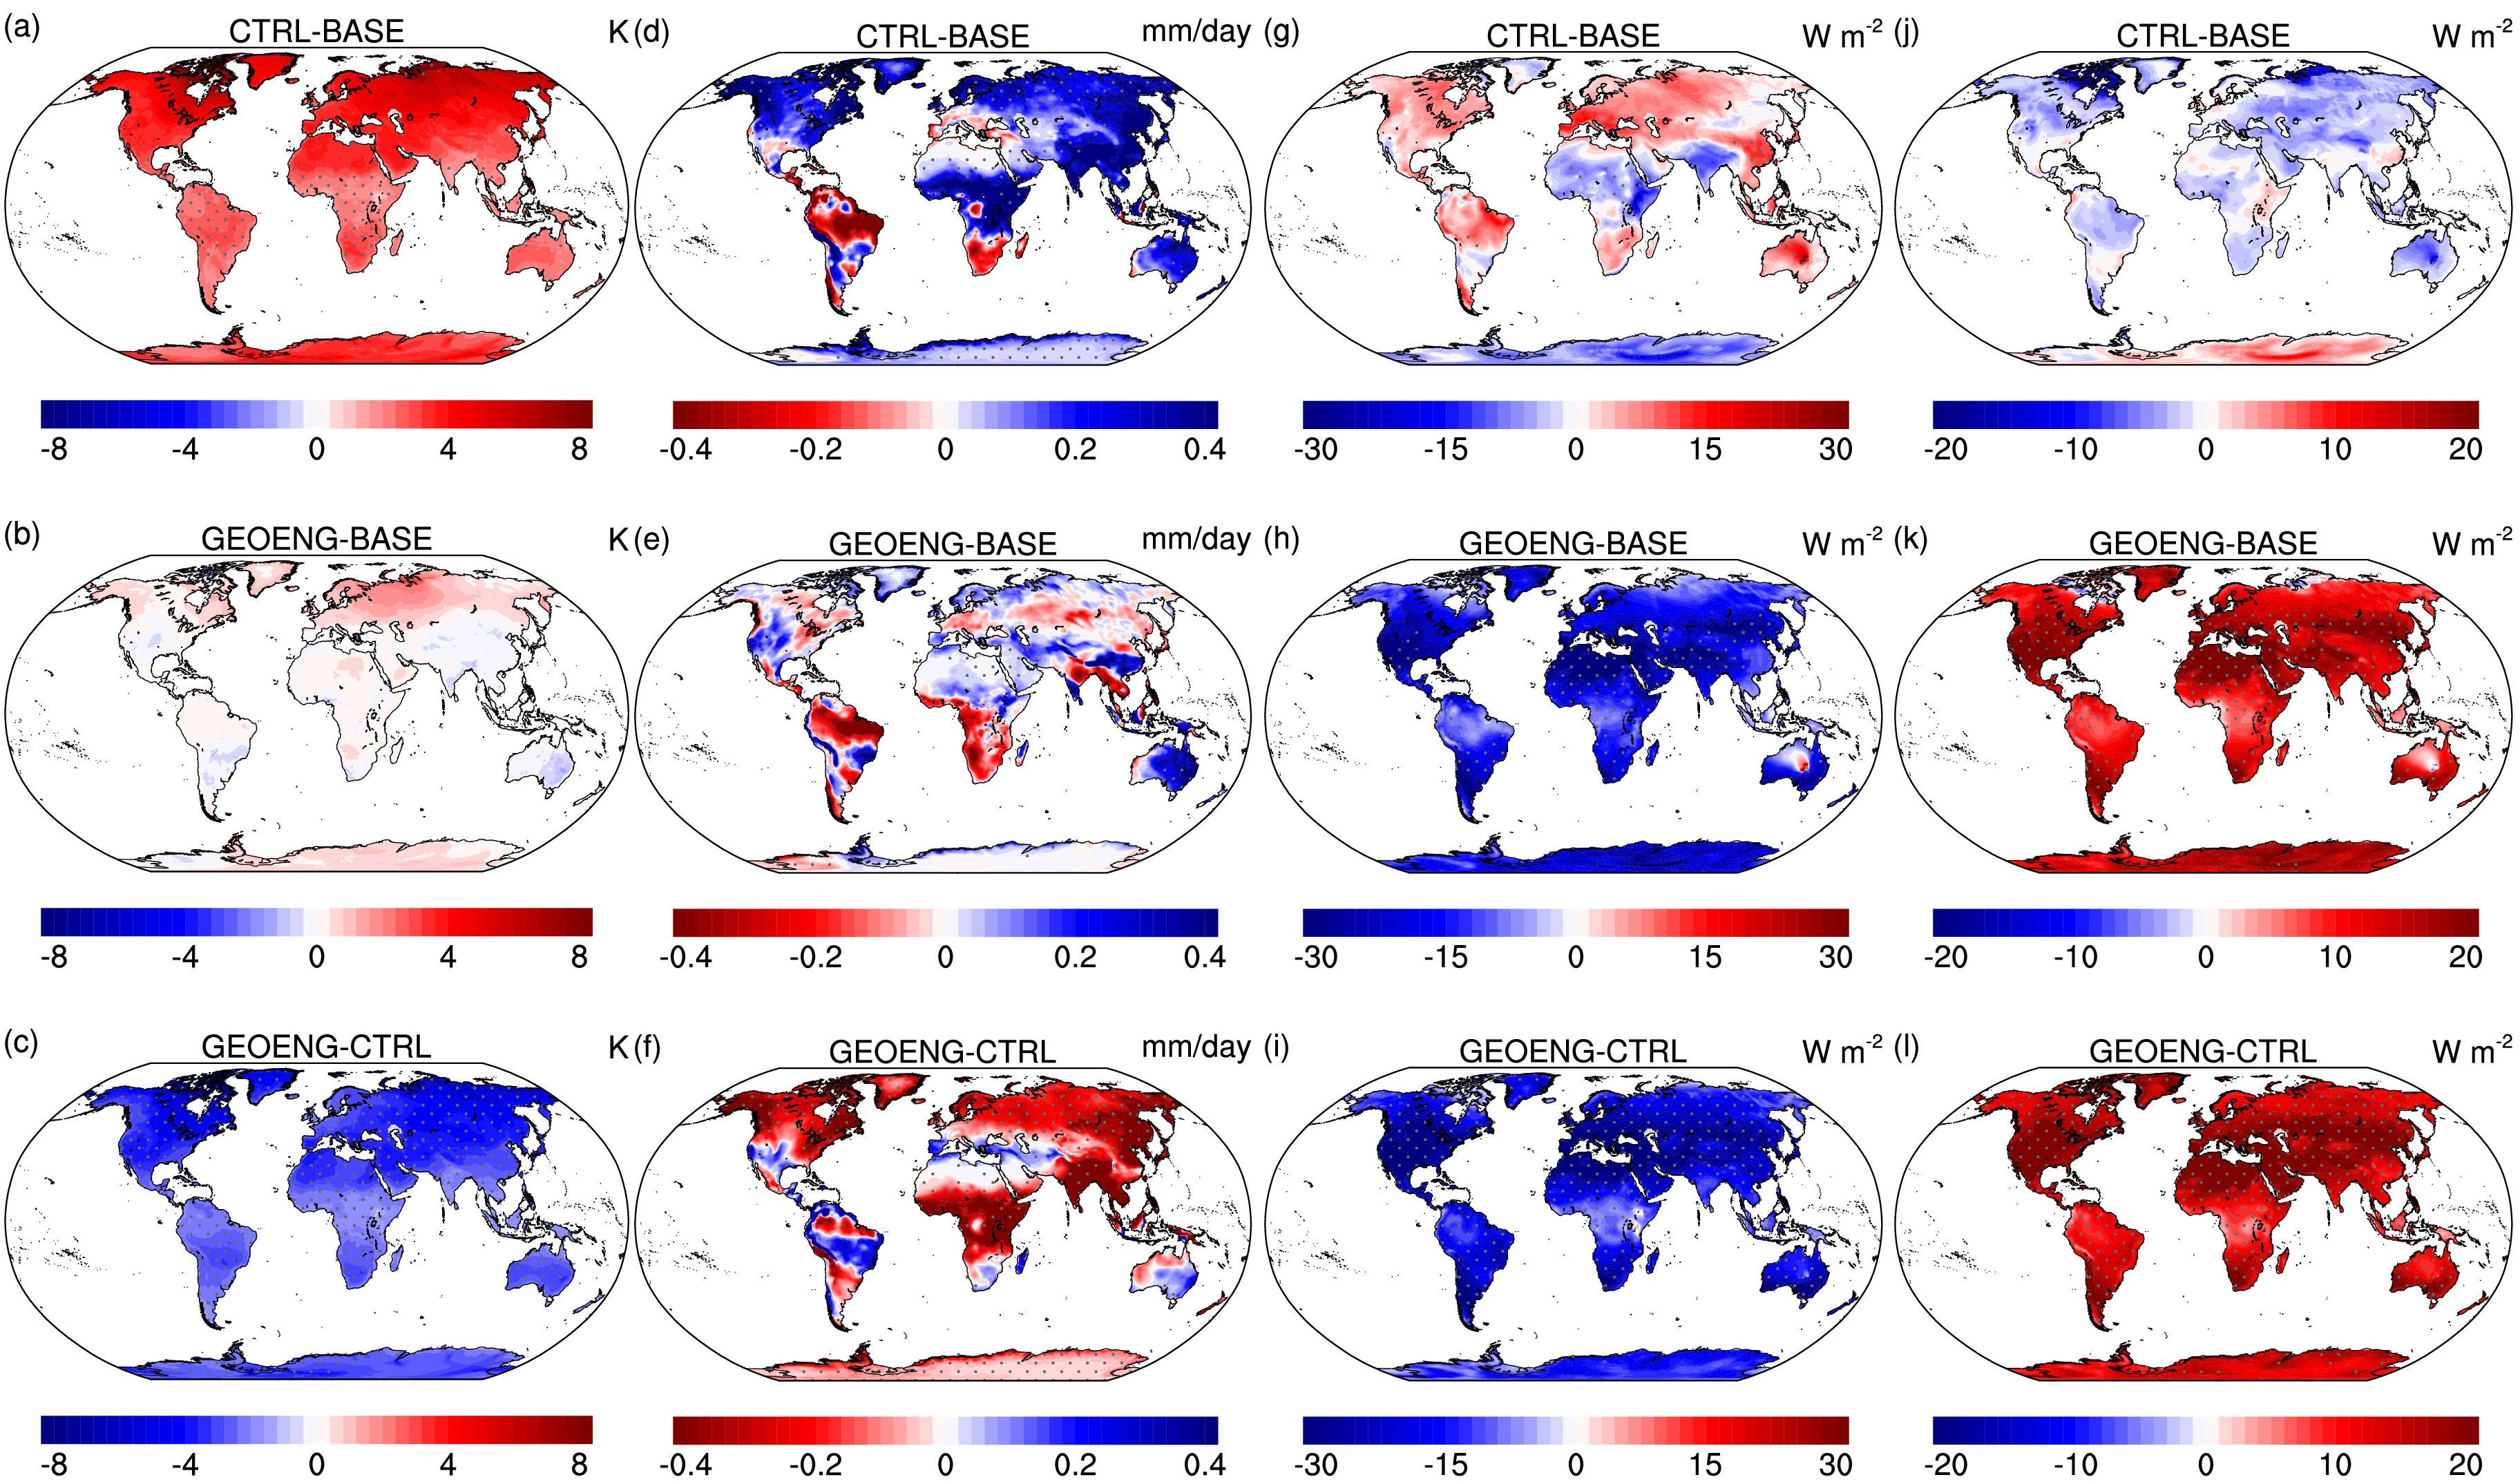
\includegraphics[width=\columnwidth]{erl_figures/Fig2.jpg}
	\end{center}
	\caption{Changes of spatial distributions between CTRL and BASE (top row), between GEOENG and BASE (middle row), and between GEOENG and CTRL (bottom row) for surface temperature (K, (a)--(c)), precipitation (mm\,day$^{-1}$, (d)--(f)), total downward direct solar radiation at the surface (W\,m$^{-2}$, (g)--(i)), and total downward diffuse solar radiation at the surface (W\,m$^{-2}$, (j)--(l)). The spatial distribution of CTRL is from the 2020--2097 time-averaged results without geoengineering while that of GEOENG is from the 2020--2097 time-averaged results with geoengineering applied. The spatial distribution of BASE is from the 2010--2019 time-average results. Light grey stippling (dots) indicates regions where the change is significant using the Student's t-test ($p < 0.1$).
		% https://iopscience.iop.org/article/10.1088/1748-9326/abacf7
	}\label{fig:geoeng_climate}
\end{figure}

\begin{itemize}
	\item Differences in climate variables (surface temperature, precipitation, and downward direct and diffuse solar radiation at the surface) were evaluated (Figure~\ref{fig:geoeng_climate}).
	\item Similarly, differences in terrestrial productivity variables (photosynthesis rate, gross primary production, net primary production, and net biome production) were assessed to characterize responses and feedbacks of the SAI treatment (Figure~\ref{fig:geoeng_bgc}).
\end{itemize}


\begin{figure}
	\begin{center}
		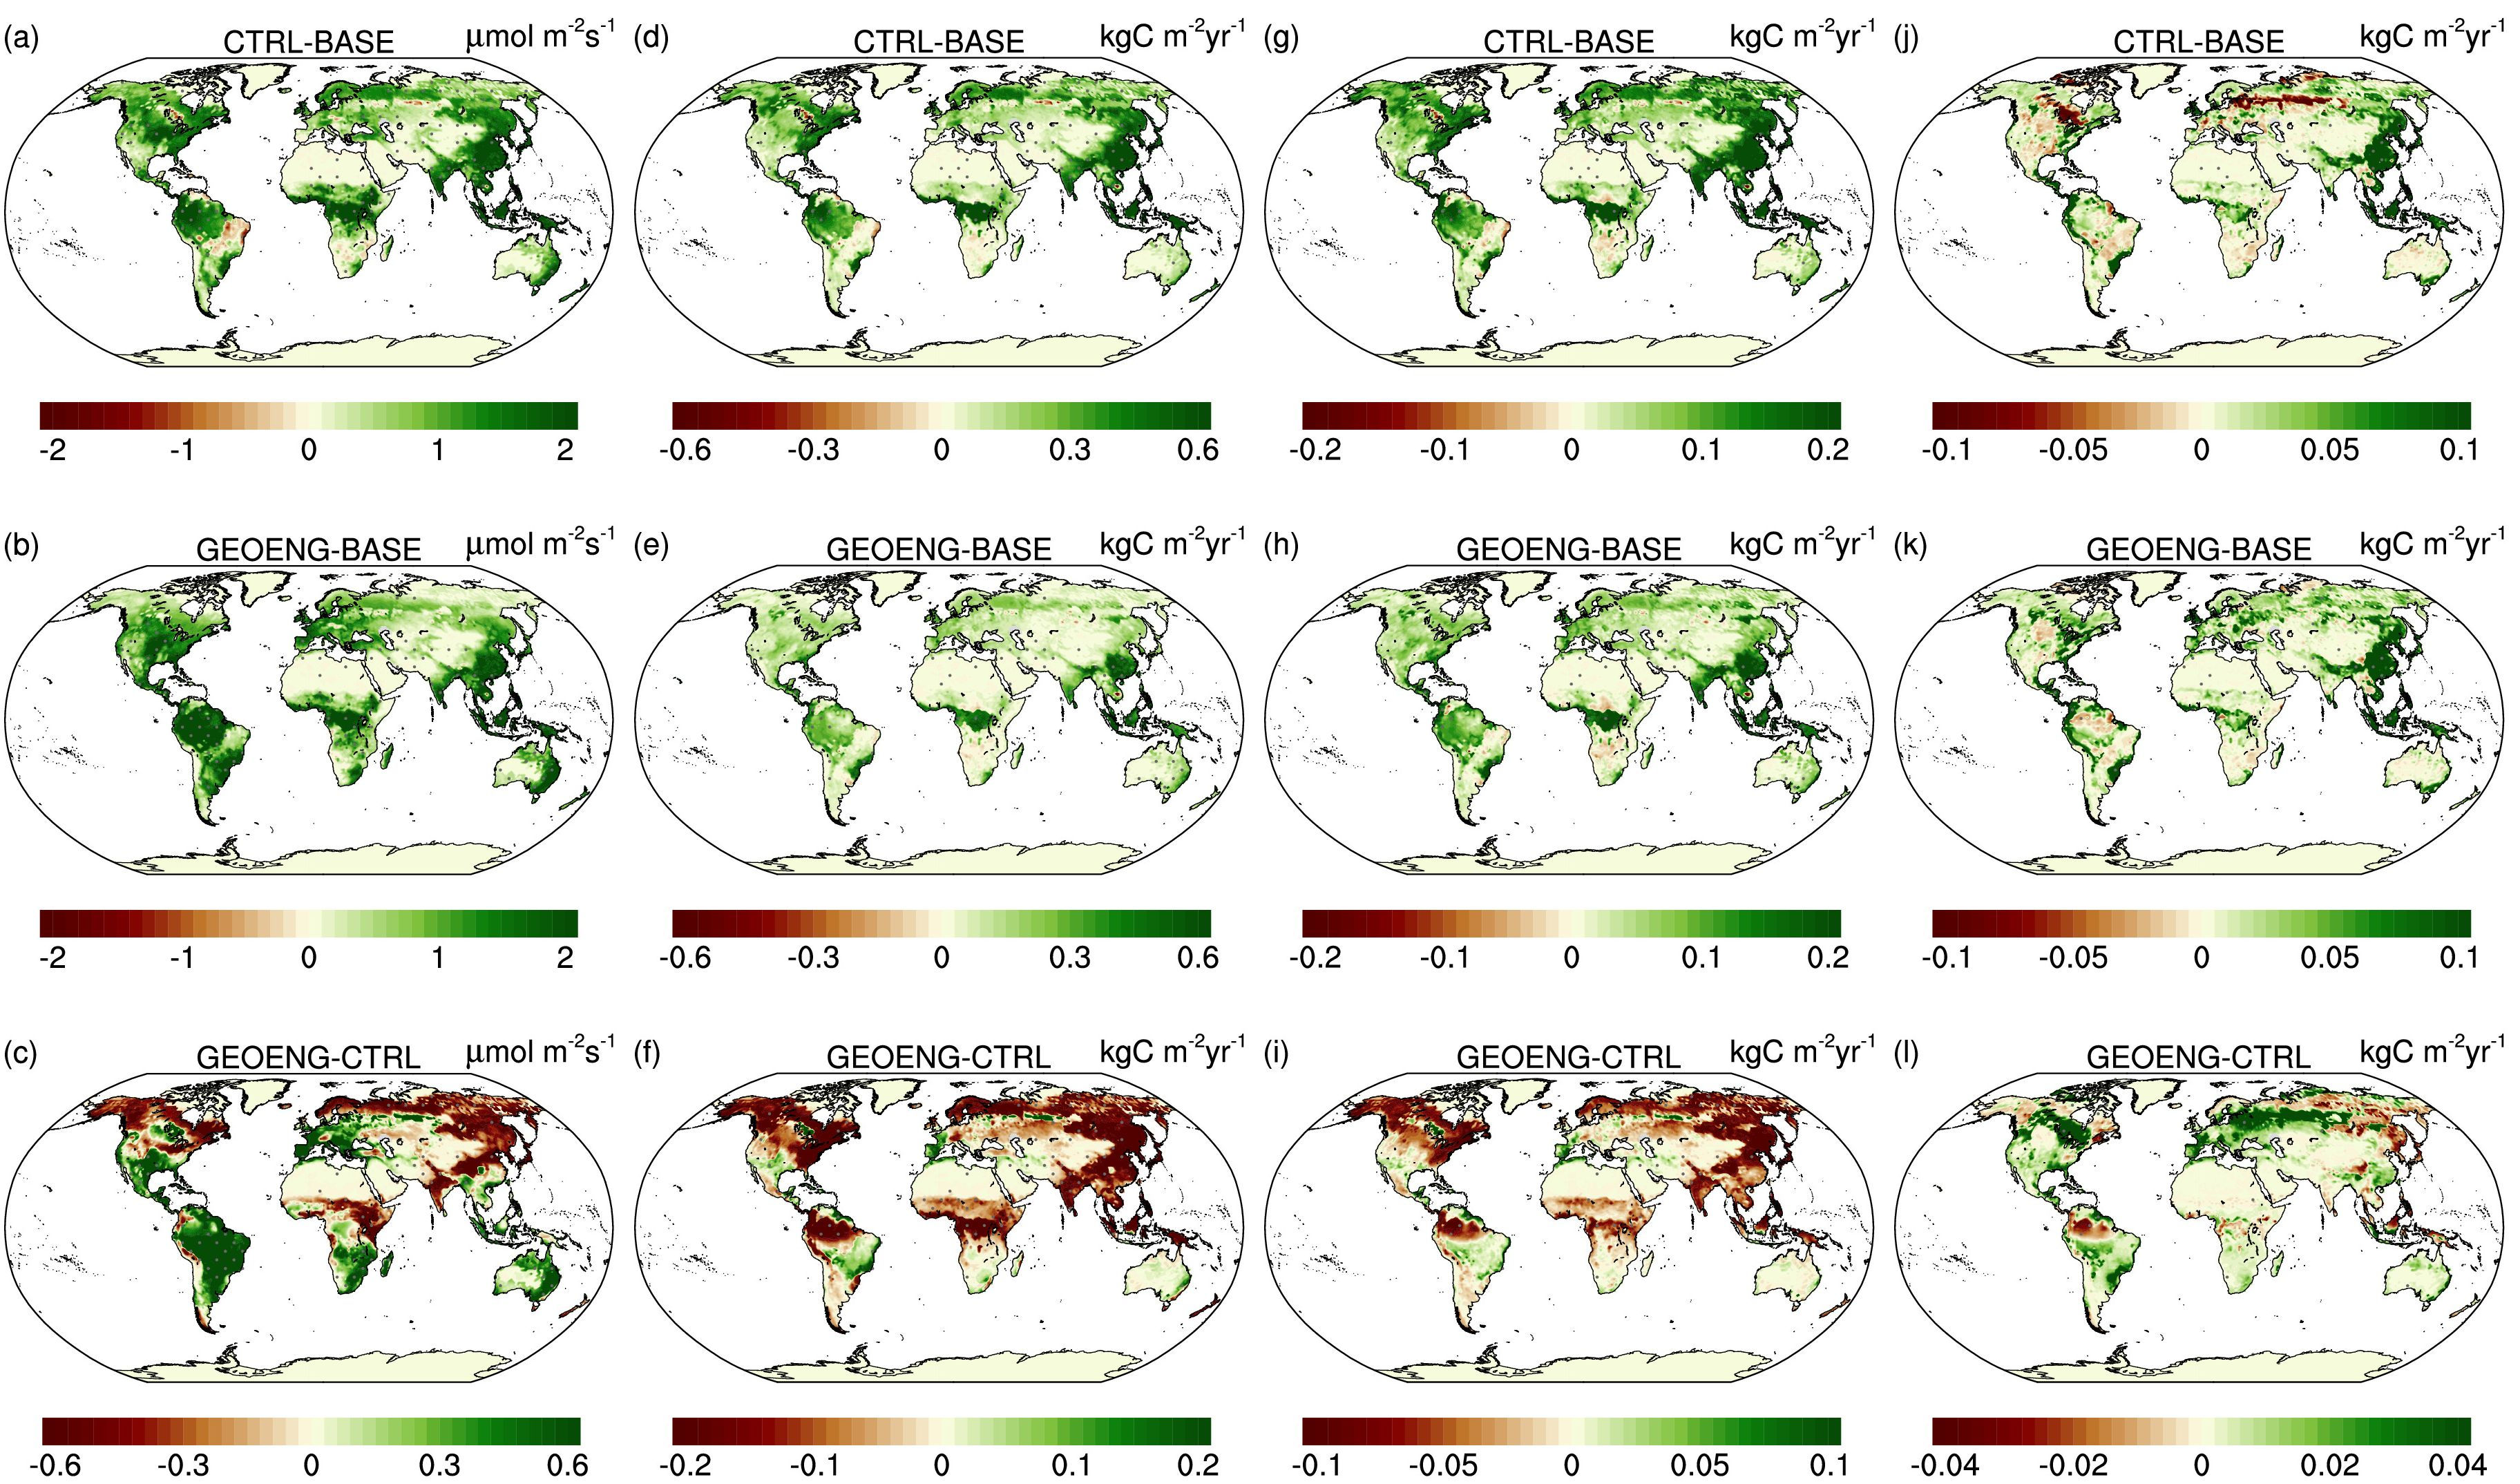
\includegraphics[width=\columnwidth]{erl_figures/Fig3.jpg}
	\end{center}
	\caption{Changes of spatial distributions between CTRL and BASE (top row), between GEOENG and BASE (middle row), and between GEOENG and CTRL (bottom row) for photosynthesis rates (µmol\,m$^{-2}$\,s$^{-1}$, (a)--(c)), gross primary production (kg\,C\,m$^{-2}$\,yr$^{-1}$, (d)--(f)), net primary production (kg\,C\,m$^{-2}$\,yr$^{-1}$, (g)--(i)), and net biome production (kg\,C\,m$^{-2}$\,yr$^{-1}$, (j)--(l)). The spatial distribution of CTRL is from the 2020--2097 time-averaged results without geoengineering while that of GEOENG is from the 2020--2097 time-averaged results with geoengineering applied. The spatial distribution of BASE is from the 2010--2019 time-average results. Light grey stippling (dots) indicates regions where the change is significant using the Student's t-test ($p < 0.1$).
		% https://iopscience.iop.org/article/10.1088/1748-9326/abacf7
	}\label{fig:geoeng_bgc}
\end{figure}


\begin{itemize}
	\item The carbon sink strength on land increased under the SAI geoengineering treatment, accumulating an additional 79\,$\pm$\,6~Pg\,C on land between 2020 and 2097 (Figure~\ref{fig:geoeng_CO2_SO2}a).

	\item If the simulation had been coupled in a way that the atmospheric CO$_2$ trajectory responded to that difference in terrestrial carbon uptake, the atmospheric CO$_2$ mole fraction would have been 872~ppm instead of 909~ppm at the year 2097, absent ocean feedbacks not incorporated into the simulations (Figure~\ref{fig:geoeng_CO2_SO2}b).

	\item Using a simple linear model, we estimated that the additional land carbon sink in the simulation would have lowered surface temperature by about 0.14$^\circ$C at 2097, again assuming no ocean interactions (Figure~\ref{fig:geoeng_CO2_SO2}c).

	\item We further estimated that sulfur injection rates could have been slightly adjusted to instead maintain a constant global temperature (Figure~\ref{fig:geoeng_CO2_SO2}d).
\end{itemize}

\begin{figure}
	\begin{center}
		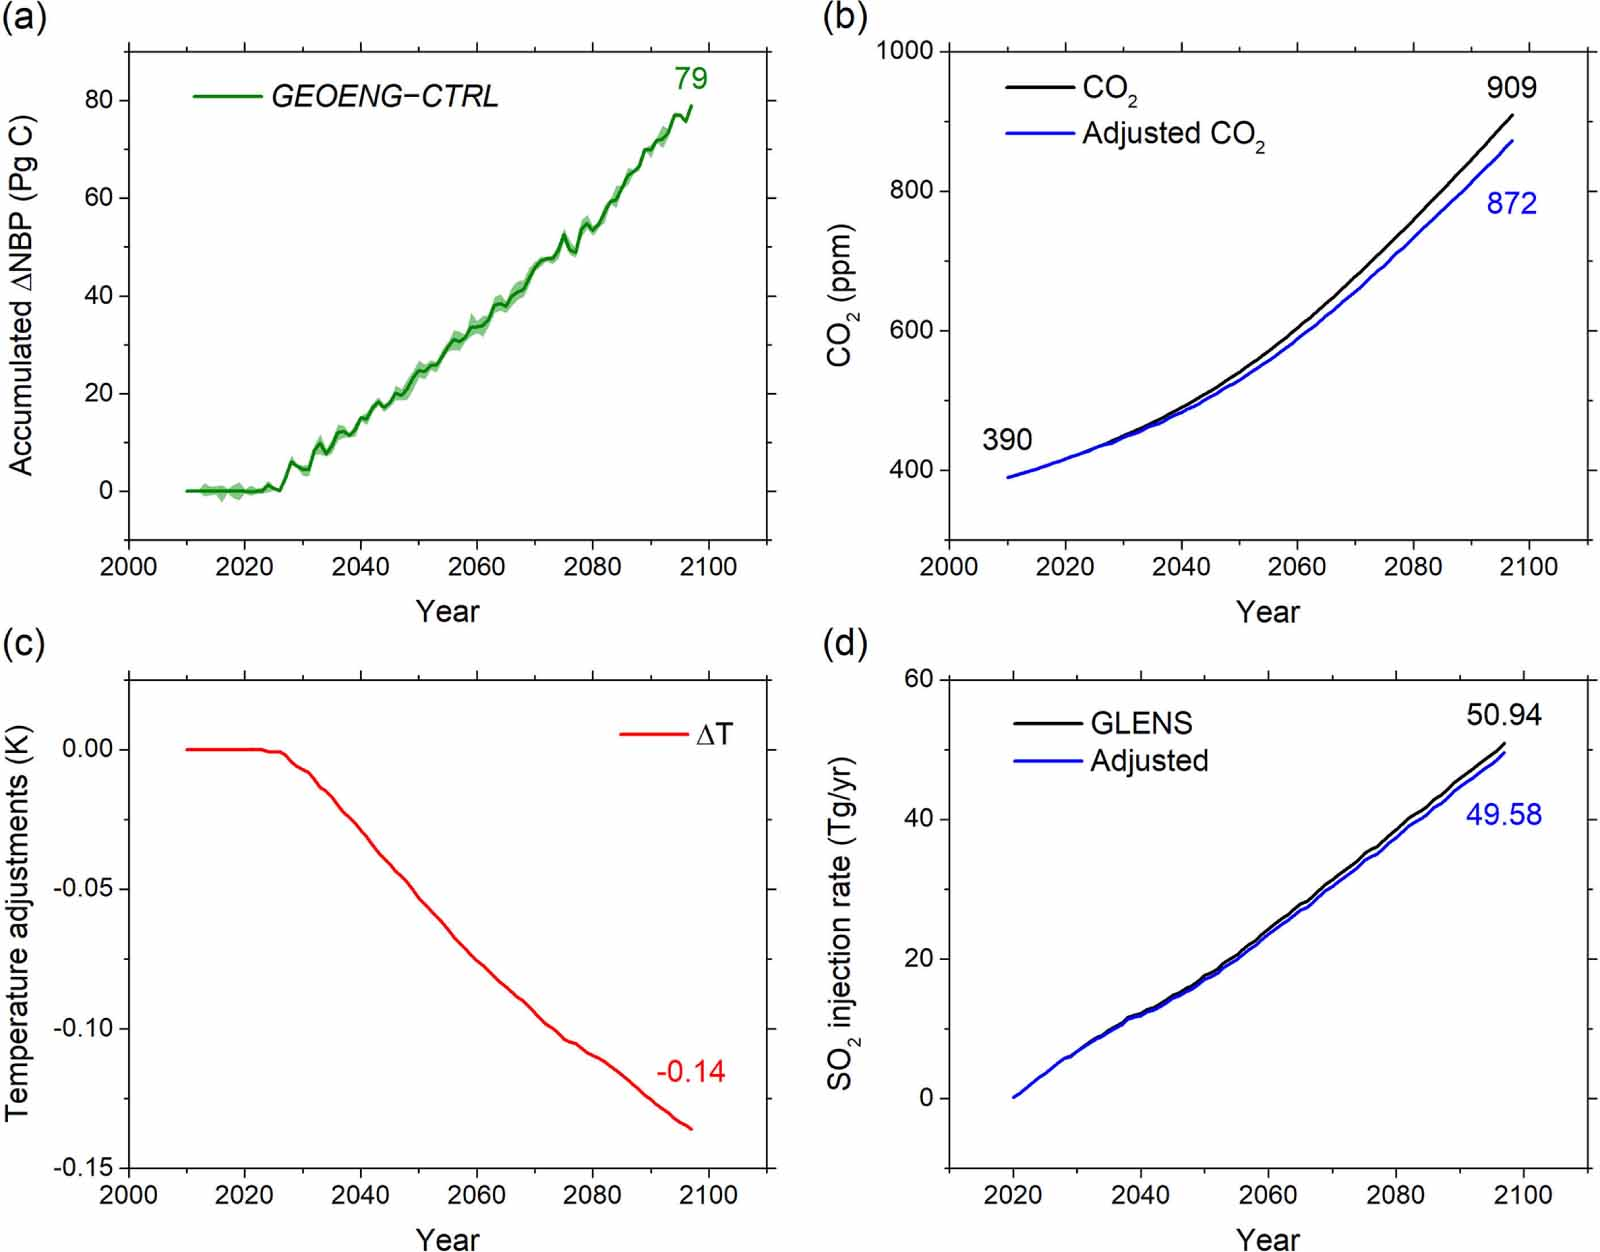
\includegraphics[width=\columnwidth]{erl_figures/Fig4.jpg}
	\end{center}
	\caption{The trajectories of (a) accumulated global carbon sink strength changes (Pg\,C) due to geoengineering, (b) the atmospheric CO$_2$ mole fraction (ppm) during 2010--2097 for BASE+CTRL (black line) and the adjusted atmospheric CO$_2$ mole fraction due to terrestrial BGC feedbacks under geoengineering (blue line), (c) surface temperature responses (K) due to atmospheric CO$_2$ adjustments, and (d) sulfur injection rates (Tg\,yr$^{-1}$) in GLENS (red) and adjusted injection rates due to terrestrial BGC feedbacks (blue).
		% https://iopscience.iop.org/article/10.1088/1748-9326/abacf7
	}\label{fig:geoeng_CO2_SO2}
\end{figure}

\begin{itemize}
	\item This study showed that a geoengineering mitigation strategy with SAI under a high greenhouse gas emission scenario would have increased land carbon storage by 79~Pg\,C globally, primarily as a result of lower ecosystem respiration and diminished disturbance effects under the SAI treatment.

	\item \textbf{Fully coupled emissions-forced simulations with interactive terrestrial and marine biogeochemistry are required to quantify competing feedback effects.}
\end{itemize}


\null\vskip0.30in

%%%%%%%%%%%%%%%%%%%%%%%%%%%%%%%%%%%%%%%%%%%%%%%%%%%%%%%%%%%%%%%%%%%%%%%%%%%%%%%
%\section*{\large Climate Intervention Research Needs}
\section*{\large National Academies Report Calls for Climate Intervention Research}
%%%%%%%%%%%%%%%%%%%%%%%%%%%%%%%%%%%%%%%%%%%%%%%%%%%%%%%%%%%%%%%%%%%%%%%%%%%%%%%

\begin{multicols}{2}
	\begin{minipage}[c]{\columnwidth}\centering
		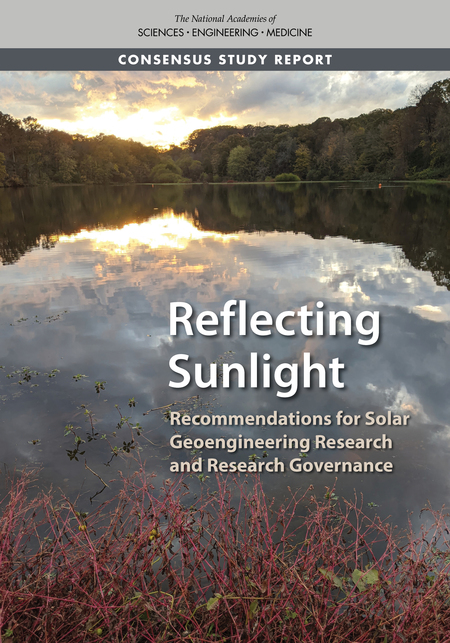
\includegraphics[width=0.8\columnwidth]{figures/25762-0309676053-450.jpg} \\
		\medskip
		\vbox{\large\textcolor{blue}{https://doi.org/10.17226/25762}}
\end{minipage}

\begin{minipage}[c]{\columnwidth}
\vbox{\large\textit{A 2021 report from the National Academies of Sciences, Engineering, and Medicine (NASEM) concludes a \textbf{strategic investment in research is needed} to enhance policymakers' understanding of climate response options. The United States should develop a transdisciplinary research program, in collaboration with other nations, to advance understanding of solar geoengineering's technical feasibility and effectiveness, possible impacts on society and the environment, and social dimensions such as public perceptions, political and economic dynamics, and ethical and equity considerations.}}
\end{minipage}
\end{multicols}



\null\vskip0.30in

%%%%%%%%%%%%%%%%%%%%%%%%%%%%%%%%%%%%%%%%%%%%%%%%%%%%%%%%%%%%%%%%%%%%%%%%%%%%%%%
\section*{\large Large-Scale Simulation Approach to Informing Policymakers}
%%%%%%%%%%%%%%%%%%%%%%%%%%%%%%%%%%%%%%%%%%%%%%%%%%%%%%%%%%%%%%%%%%%%%%%%%%%%%%%

%\input{gpp_change}

%\null\vskip-0.60in
\begin{itemize}
	\item To fill the nationally recognized research gap in understanding potential Earth system feedbacks of SAI on ecosystems, regional atmospheric circulation, and biogeochemical cycles, we will conduct a series of increasingly complex geoengineering simulations, using \textbf{DOE's Energy Exascale Earth System Model (E3SM)}.

	\item \textbf{These simulations will mimic the effects of CDR, SAI, and CDR plus SAI in combination.}

	\item We will start with the well-defined SSP5-3.4-OS mid-range overshoot CO$_2$ trajectory from CMIP6, which prescribes a drawdown of atmospheric CO$_2$ due to CDR, large reductions in emissions, or both.

	\item In that scenario, global surface temperatures rise by $>$2.5$^\circ$C around 2040, \textbf{well above the 2$^\circ$C threshold that may induce irreversible impacts}.

	\item A second set of simulations would introduce SAI to simultaneously cool the surface, or \textbf{``shave'' the temperature peak}, until drawdown is sufficient to assure $<$2$^\circ$ warming at any time as illustrated in Figure~\ref{fig:peak_shaving}B.
\end{itemize}

\begin{figure}
	\begin{center}
		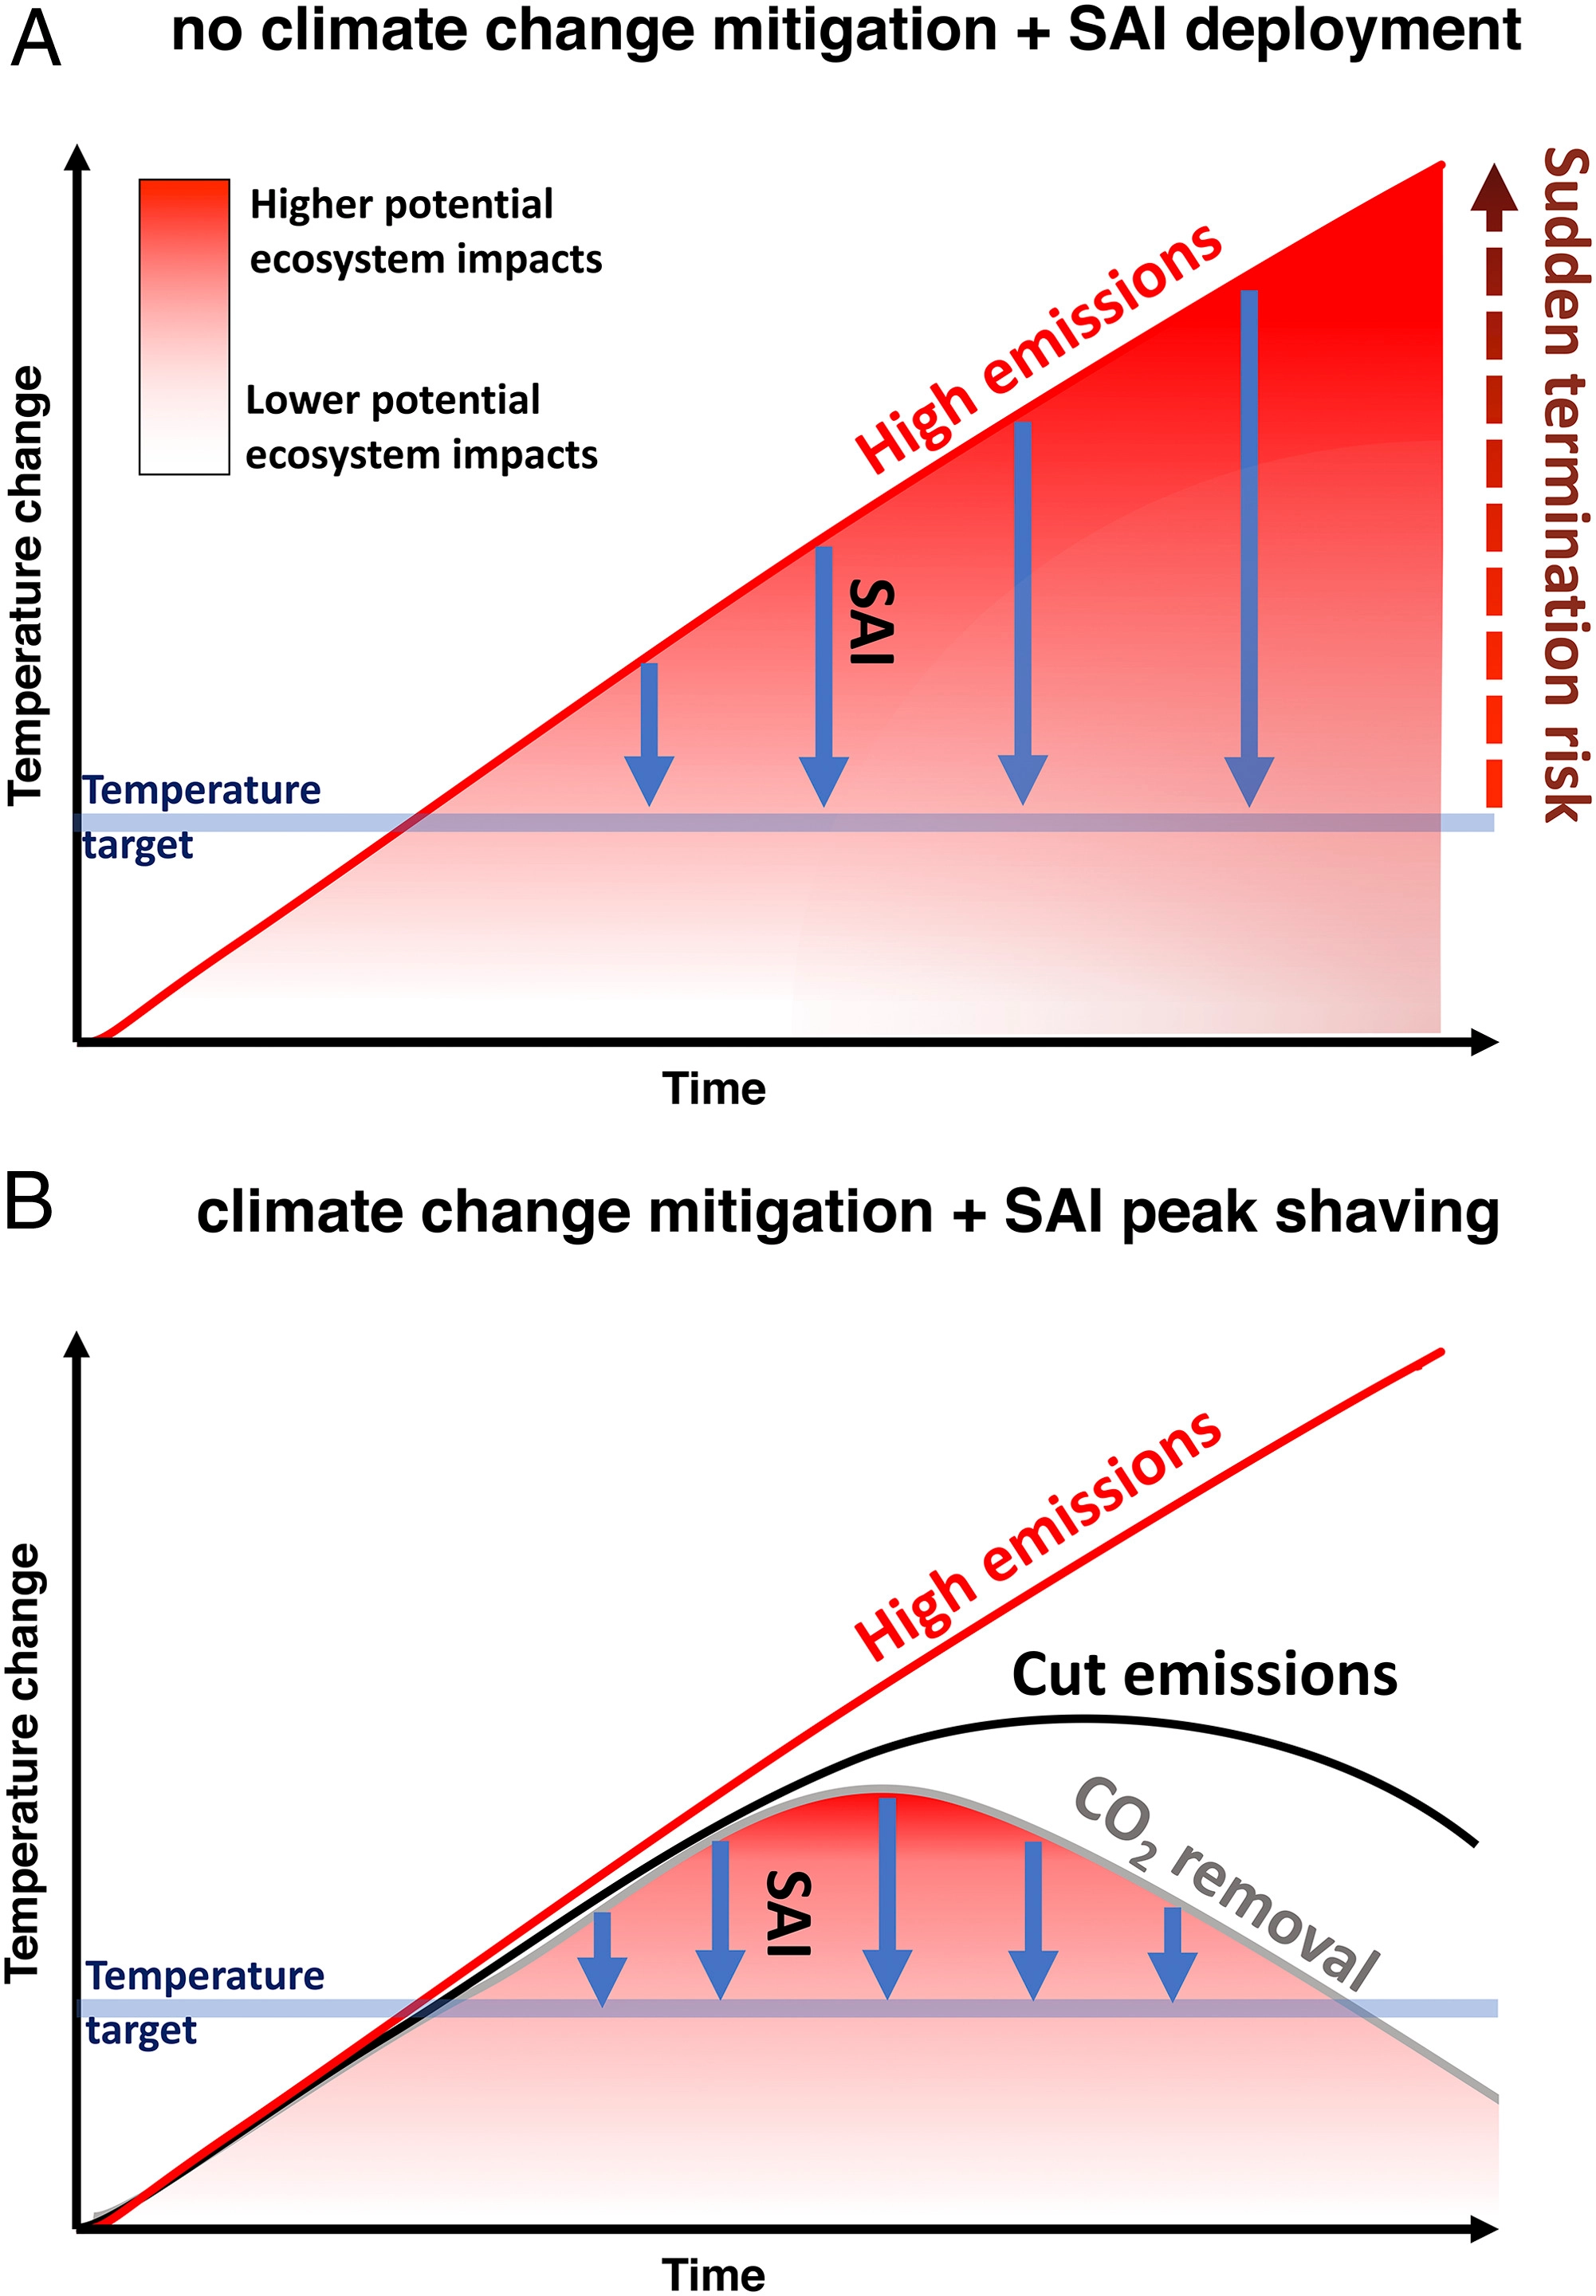
\includegraphics[trim=0cm 52.0cm 0cm 0cm,clip=true,width=0.48\columnwidth]{figures/pnas_fig2.png} \hfill
		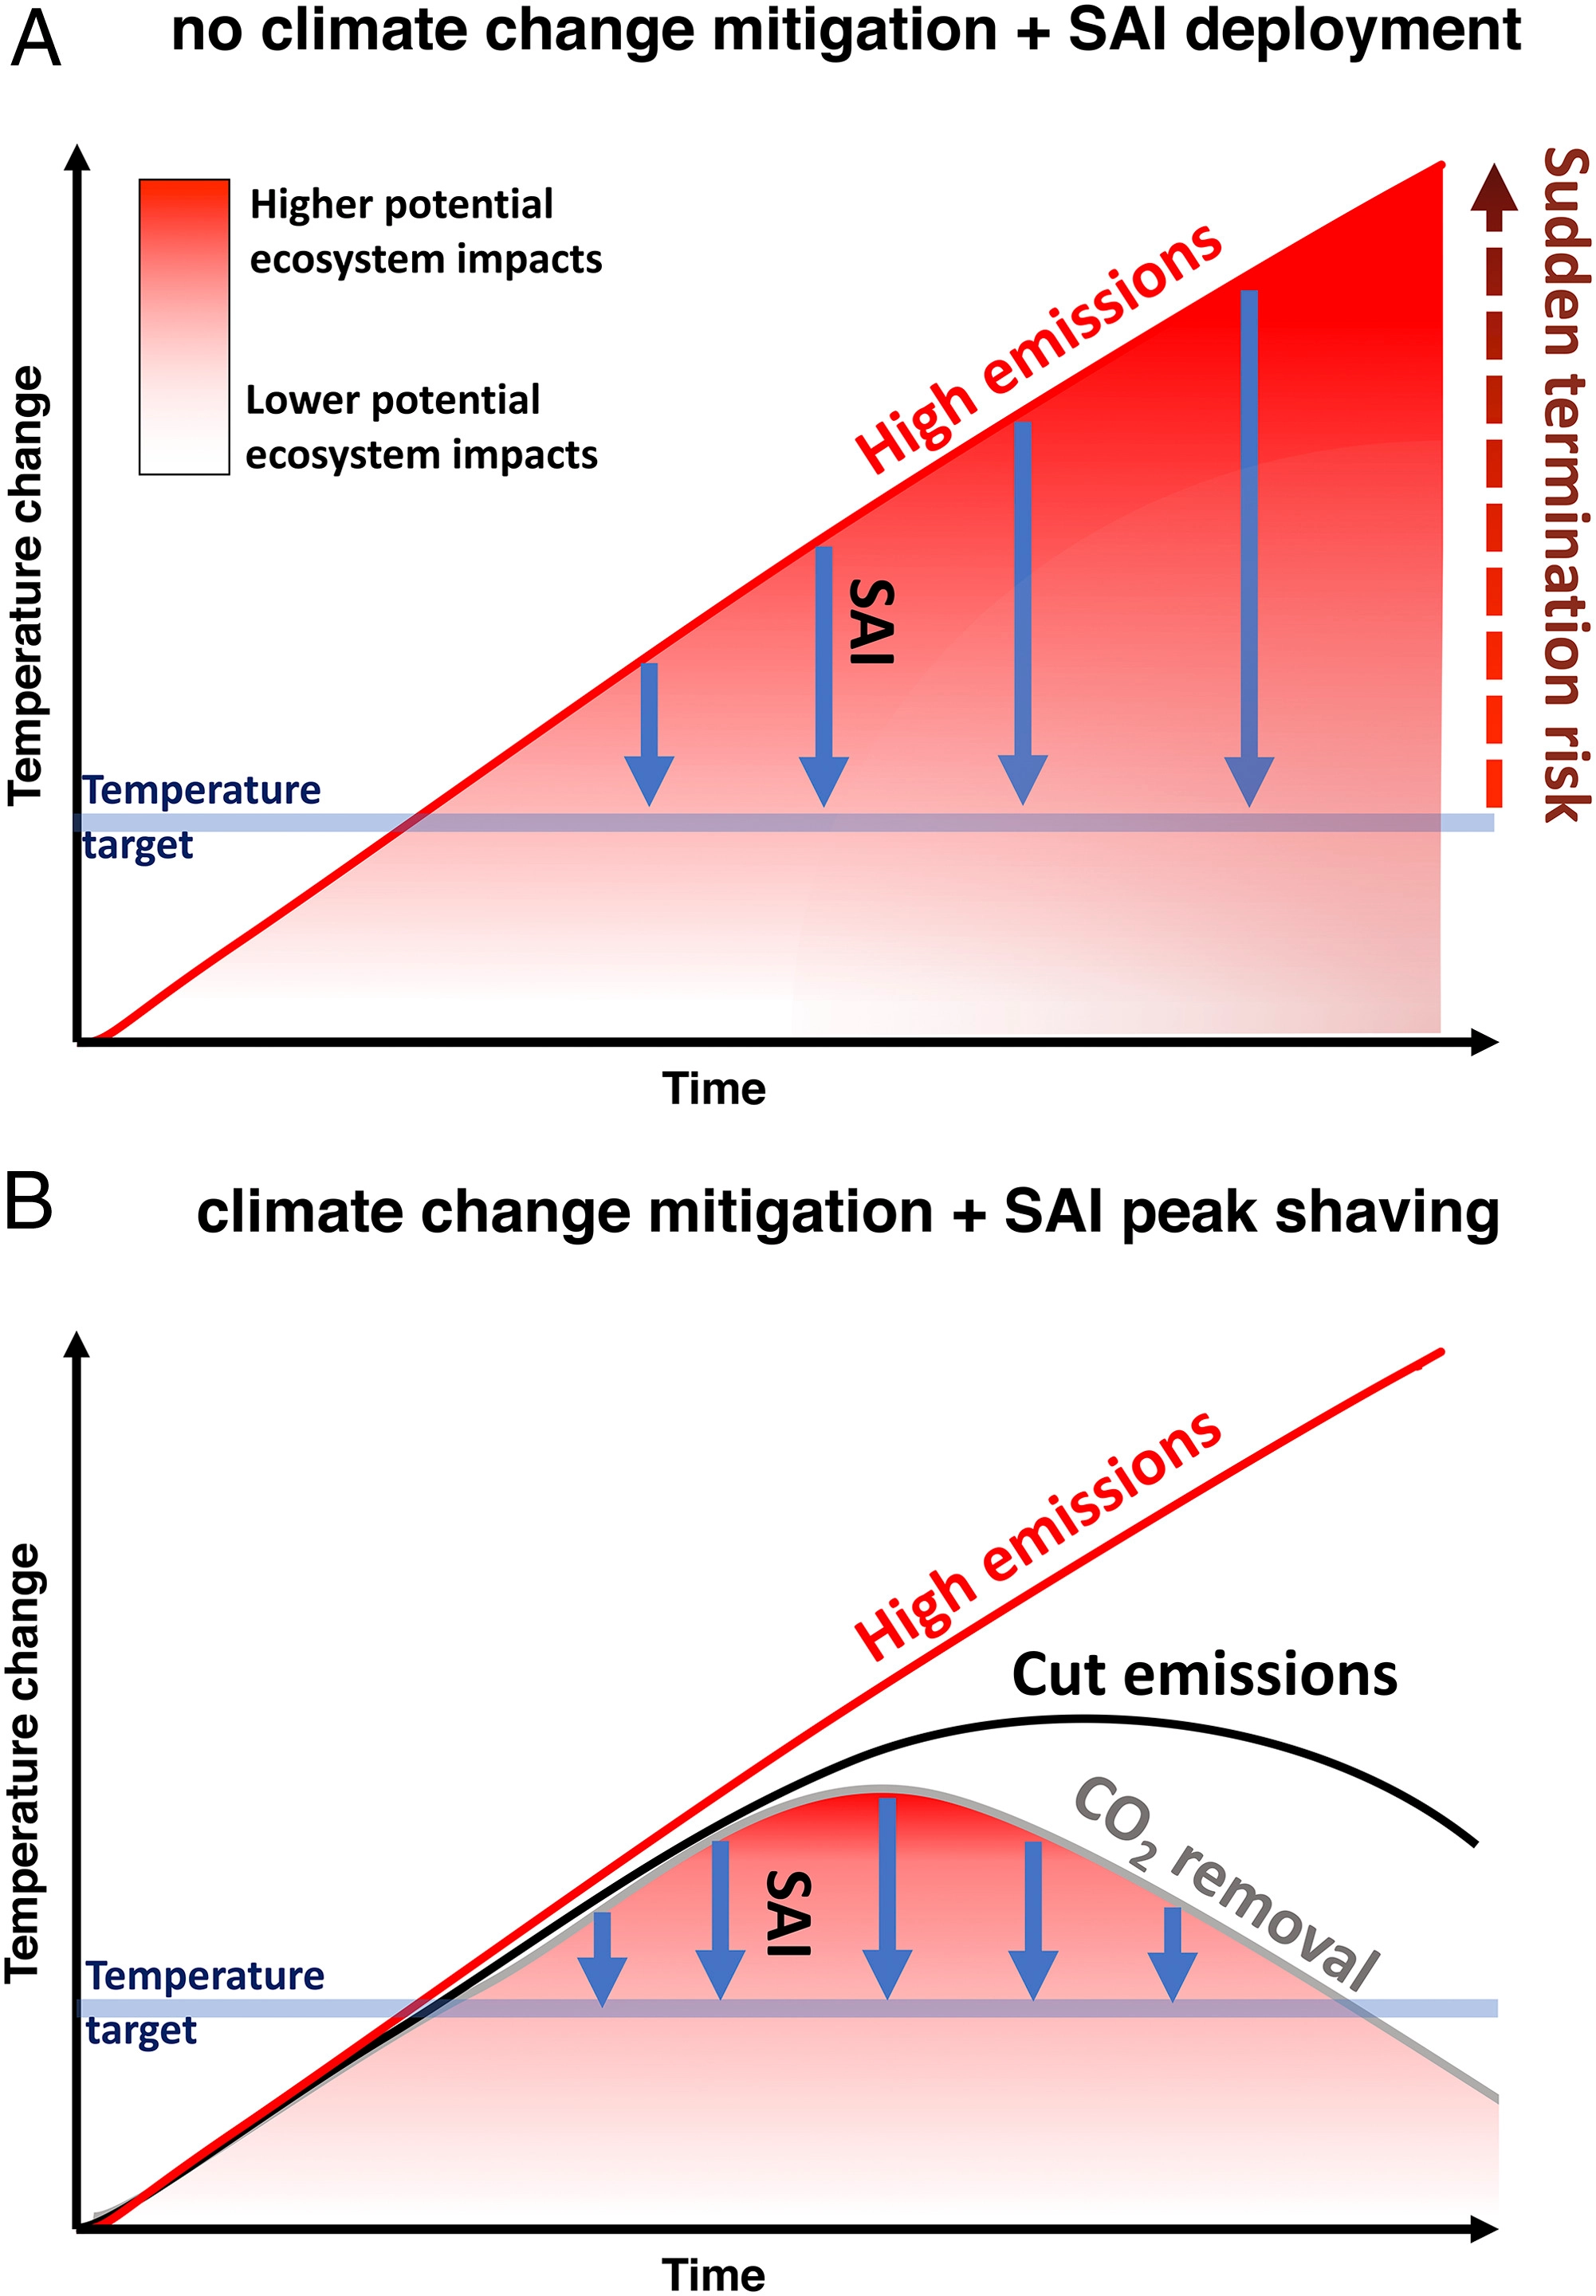
\includegraphics[trim=0cm 0cm 0cm 51.89cm,clip=true,width=0.48\columnwidth]{figures/pnas_fig2.png}
	\end{center}
	\caption{Potential temperature change over time for two different SAI scenarios. (A) In a future with no climate change mitigation and with SAI deployment, high emissions result in rising temperatures (red line). Increasing amounts of SAI would have to be deployed to reduce temperature (blue arrows) to a specific temperature target (blue line). The risk of sudden SAI termination also increases (red arrow). (B) In a future with climate change mitigation and SAI ``peak shaving,'' temperature changes are first reduced by a combination of emission reduction (black line) and CDR (CO$_2$ removal, gray line), then further reduced by SAI (blue arrows). The red shaded areas below the two curves indicate the potential overall risk for ecological systems from increased temperature and SAI deployment; carbon emissions alone would not create the same degree of risk reduction as shown in B. We note that SAI is not akin to a global thermostat that would only control global temperatures to remediate GHG-induced warming. GHGs add energy to the system at the surface and throughout the atmosphere, whereas reducing sunlight with SAI only changes the energy balance at Earth's surface. Furthermore, GHGs operate 24 h a day and all year long, whereas reducing sunlight primarily has a direct impact during the daytime and more so in summer than winter. Adopted from Zarnetske et al. (2021).
		% https://www.pnas.org/doi/10.1073/pnas.1921854118
	}\label{fig:peak_shaving}
\end{figure}

\begin{itemize}
	\item \textbf{These and other scenario simulations must be performed and analyzed to determine the effects of reduced radiative forcing despite increasing atmospheric CO$_2$ levels on Earth's climate, regional atmospheric dynamics and aerosol-cloud interactions, and terrestrial and marine carbon sink strengths.}

	\item \textbf{This research will better characterize and reduce scientific and societal uncertainties concerning the benefits and risks of solar geoengineering deployment, so that informed decisions can be made in the future about possible implementation.}

\end{itemize}




%\vskip-0.25in
%%%%%%%%%%%%%%%%%%%%%%%%%%%%%%%%%%%%%%%%%%%%%%%%%%%%%%%%%%%%%%%%%%%%%%%%%%%%%%%
%\section*{\large Discussion and Conclusions}
%%%%%%%%%%%%%%%%%%%%%%%%%%%%%%%%%%%%%%%%%%%%%%%%%%%%%%%%%%%%%%%%%%%%%%%%%%%%%%%

%\vspace*{-0.25in}
%\input{discussion}

%%%%%%%%%%%%%%%%%%%%%%%%%%%%%%%%%%%%%%%%%%%%%%%%%%%%%%%%%%%%%%%%%%%%%%%%%%%%%%%
%\section*{\large Conclusions}
%%%%%%%%%%%%%%%%%%%%%%%%%%%%%%%%%%%%%%%%%%%%%%%%%%%%%%%%%%%%%%%%%%%%%%%%%%%%%%%

%%%%%%%%%%%%%%%%%%%%%%%%%%%%%%%%%%%%%%%%%%%%%%%%%%%%%%%%%%%%%%%%%%%%%%%%%%%%%%%
%\begin{itemize}
%\item Blah
%
%\end{itemize}
%%%%%%%%%%%%%%%%%%%%%%%%%%%%%%%%%%%%%%%%%%%%%%%%%%%%%%%%%%%%%%%%%%%%%%%%%%%%%%%

%%%%%%%%%%%%%%%%%%%%%%%%%%%%%%%%%%%%%%%%%%%%%%%%%%%%%%%%%%%%%%%%%%%%%%%%%%%%%%%
%\section*{\large References}
%%%%%%%%%%%%%%%%%%%%%%%%%%%%%%%%%%%%%%%%%%%%%%%%%%%%%%%%%%%%%%%%%%%%%%%%%%%%%%%

%\medskip
%\vbox{\hangindent=0.25in\hangafter=1
%Forrest M.\ Hoffman, James T.\ Randerson, Vivek K.\ Arora, Qing Bao, Patricia Cadule, Duoying Ji, Chris D.\ Jones, Michio Kawamiya, Samar Khatiwala, Keith Lindsay, Atsushi Obata, Elena Shevliakova, Katharina D.\ Six, Jerry F.\ Tjiputra, Evgeny M.\ Volodin, and Tongwen Wu (2014), Causes and implications of persistent atmospheric carbon dioxide biases in Earth System Models, \textit{J.\ Geophys.\ Res.\ Biogeosci.}, 119(2):141--162. doi: 10.1002/2013JG002381.}
%
%{
%\nocite{Hoffman_JGRB_20140201}
% \scriptsize%\rm
% \bibliographystyle{unsrtnat}
%\vskip-0.5in
% \bibliography{refs/abbrev,%
%refs/Hoffman_JGRB_20140201%
%}
%}

{
\nocite{Lawrence_NatCommun_20180913,%
Reflecting_Sunlight_2021,%
Yang_ERL_20200928,%
Zarnetske_PNAS_20210413}
%\scriptsize%\rm
\renewcommand\refname{\large References%
%\vspace{-0.75\baselineskip}
}
%\bibliographystyle{unsrtnat}
\bibliographystyle{refs/agufull08}
%\vskip-0.5in
\bibliography{refs/abbrev,%
refs/Lawrence_NatCommun_20180913,
refs/Reflecting_Sunlight_2021,
refs/Yang_ERL_20200928,
refs/Zarnetske_PNAS_20210413%
}
}

%\vspace*{-0.25in}
%%%%%%%%%%%%%%%%%%%%%%%%%%%%%%%%%%%%%%%%%%%%%%%%%%%%%%%%%%%%%%%%%%%%%%%%%%%%%%%
\section*{\large Acknowledgements}
%%%%%%%%%%%%%%%%%%%%%%%%%%%%%%%%%%%%%%%%%%%%%%%%%%%%%%%%%%%%%%%%%%%%%%%%%%%%%%%

%%%%%%%%%%%%%%%%%%%%%%%%%%%%%%%%%%%%%%%%%%%%%%%%%%%%%%%%%%%%%%%%%%%%%%%%%%%%%%%
% \begin{center}
%  \vskip-0.25in
%  
\includegraphics[width=0.50\columnwidth]{logos/DOE_Office_of_Science_logo.pdf}
%  \hskip0.50in
%  
\includegraphics[width=0.16\columnwidth]{logos/USFS_Logo.png}
% \end{center}

\vspace*{-0.15in}
%\smallskip
\vbox{%\small
This research is supported by the Oak Ridge National Laboratory (ORNL)
Laboratory Director's Reserach and Development (LDRD) Fund.
Additional support was provided by the Reducing Uncertainties in
Biogeochemical Interactions through Synthesis and Computation (RUBISCO)
Science Focus Area, which is sponsored by the Regional and Global Model
Analysis (RGMA) activity of the Earth \& Environmental Systems Modeling
(EESM) Program in the Earth and Environmental Systems Sciences Division
(EESSD) of the Office of Biological and Environmental Research (BER)
in the US Department of Energy Office of Science.
%
The Climate Intervention Biology Working Group is funded by the National
Science Foundation (1937619, PI: J. Gurevitch; 1937699, PI: P. Zarnetske).
%
This research used resources of the Oak Ridge Leadership Computing
Facility (OLCF) at Oak Ridge National Laboratory (ORNL), which is managed
by UT-Battelle, LLC, for the US Department of Energy under Contract
No.\ DE-AC05-00OR22725.
%
%The Lawrence Berkeley National Laboratory is managed by the University
%of California for the U.\ S.\ Department of Energy under Contract No.\
%DE-AC02-05CH11231.
%
%The National Center for Atmospheric Research (NCAR) is sponsored primarily
%by the National Science Foundation.
%
%The United States Government retains and the publisher, by accepting the
%article for publication, acknowledges that the United States Government
%retains a non-exclusive, paid-up, irrevocable, world-wide license to
%publish or reproduce the published form of this manuscript, or allow
%others to do so, for United States Government purposes.
%
%We acknowledge the World Climate Research Programme's Working Group
%on Coupled Modelling, which is responsible for CMIP, and we thank the
%climate modeling groups (listed in Table~1 of this
%poster) for producing and making available their model output. For CMIP
%the U.\ S.\ Department of Energy's Program for Climate Model Diagnosis
%and Intercomparison provides coordinating support and led development
%of software infrastructure in partnership with the Global Organization
%for Earth System Science Portals.
}

%%%%%%%%%%%%%%%%%%%%%%%%%%%%%%%%%%%%%%%%%%%%%%%%%%%%%%%%%%%%%%%%%%%%%%%%%%%%%%%

%\vfill
%%%%%%%%%%%%%%%%%%%%%%%%%%%%%%%%%%%%%%%%%%%%%%%%%%%%%%%%%%%%%%%%%%%%%%%%%%%%%%%
%{\Large\centering
%\begin{tabular}{b{0.77\columnwidth} c}
%  \textcolor{blue}{\textbf{Want a copy of this poster to read later?  Just scan this QR code with your smartphone!}} & \\ %\includegraphics[width=0.2\columnwidth]{figures/qrcode.22265053.png} \\
%\end{tabular}
%}
%%%%%%%%%%%%%%%%%%%%%%%%%%%%%%%%%%%%%%%%%%%%%%%%%%%%%%%%%%%%%%%%%%%%%%%%%%%%%%%

\end{multicols}
\end{document} 
